%% ----------------------------------------------------------------
%% Thesis.tex -- MAIN FILE (the one that you compile with LaTeX)
%% ---------------------------------------------------------------- 

% Set up the document
\documentclass[a4paper, 11pt, oneside]{Thesis}  % Use the "Thesis" style, based on the ECS Thesis style by Steve Gunn
\usepackage{indentfirst}
\graphicspath{Figures/}  % Location of the graphics files (set up for graphics to be in PDF format)

% Include any extra LaTeX packages required
\usepackage[square, numbers, comma, sort&compress]{natbib}  % Use the "Natbib" style for the references in the Bibliography
\usepackage{verbatim}  % Needed for the "comment" environment to make LaTeX comments
\usepackage{vector}  % Allows "\bvec{}" and "\buvec{}" for "blackboard" style bold vectors in maths
\usepackage{graphicx}
\hypersetup{urlcolor=blue, colorlinks=true}  % Colours hyperlinks in blue, but this can be distracting if there are many links.
\setlength{\parindent}{4em}
\setlength{\parskip}{1em}

\usepackage{multirow}

%% ----------------------------------------------------------------
\begin{document}

\frontmatter      % Begin Roman style (i, ii, iii, iv...) page numbering

% Set up the Title Page
\title  {A semi-assembly approach for genome reconstruction using
closely-related reference sequences}
\authors  {\texorpdfstring
            {\textbf{{Yu-Ting Sun}}}
            {Yu-Ting Sun}
            }
%\addresses  {\groupname\\\deptname\\\univname}  % Do not change this here, instead these must be set in the "Thesis.cls" file, please look through it instead
\date       {\today}
\subject    {}
\keywords   {}

\maketitle
%% ----------------------------------------------------------------

\setstretch{1.3}  % It is better to have smaller font and larger line spacing than the other way round

% Define the page headers using the FancyHdr package and set up for one-sided printing
\fancyhead{}  % Clears all page headers and footers
\rhead{\thepage}  % Sets the right side header to show the page number
\lhead{}  % Clears the left side page header

\pagestyle{fancy}  % Finally, use the "fancy" page style to implement the FancyHdr headers


%------------------


%------------------



% The Abstract Page
%\addtotoc{Abstract}  % Add the "Abstract" page entry to the Contents
%\abstract{
%\addtocontents{toc}{\vspace{1em}}  % Add a gap in the Contents, for aesthetics
%\chapter{Abstract}

In recent years, as many genomes have been sequenced and assembled, the newly-sequenced genomes are often closely-related to an existing genome. However, owing to complex repeat structures in the genome, the genomes assembled by existing methods are often highly fragmented. In this thesis, we design a semi-assembly approach (called SemiAssembler) which integrate reference-mapping approaches and {\em de novo} assembly to reconstruct a newly-sequenced genome using closely-related genome sequences. A draft genome is first created by adding (removing) inter-species insertions (deletions) to (from) the related genome, respectively. Subsequently, the draft genome sequence is replaced with the contig sequences assembled from short reads, which aims to reflect inter-species SNPs and small-sized indels. Simulation results indicated our method has high precision and recall rates. The program is used to assemble two $O. Sativa$ genomes. A substantial amount of large insertions/deletions and small indels found by our method were validated by PCR.

Keywords:{\em de novo} assembly, closely-related genome sequences
%}

%\clearpage  % Abstract ended, start a new page


%% ----------------------------------------------------------------

\setstretch{1.3}  % Reset the line-spacing to 1.3 for body text (if it has changed)

% The Acknowledgements page, for thanking everyone
%\acknowledgements{
%\addtocontents{toc}{\vspace{1em}}  % Add a gap in the Contents, for aesthetics

%The acknowledgements and the people to thank go here, don't forget to include your project advisor\ldots

%}
%\clearpage  % End of the Acknowledgements
%% ----------------------------------------------------------------

%%\pagestyle{fancy}  %The page style headers have been "empty" all this time, now use the "fancy" headers as defined before to bring them back


%% ----------------------------------------------------------------
%%\lhead{\emph{Contents}}  % Set the left side page header to "Contents"
%\tableofcontents  % Write out the Table of Contents

%% ----------------------------------------------------------------
%%\lhead{\emph{List of Figures}}  % Set the left side page header to "List if Figures"
%\listoffigures  % Write out the List of Figures

%% ----------------------------------------------------------------
%%\lhead{\emph{List of Tables}}  % Set the left side page header to "List of Tables"
%\listoftables  % Write out the List of Tables

%% ----------------------------------------------------------------
%%\setstretch{1.5}  % Set the line spacing to 1.5, this makes the following tables easier to read
%%\clearpage  % Start a new page
%%\lhead{\emph{Abbreviations}}  % Set the left side page header to "Abbreviations"
%%\listofsymbols{ll}  % Include a list of Abbreviations (a table of two columns)
%%{
% \textbf{Acronym} & \textbf{W}hat (it) \textbf{S}tands \textbf{F}or \\
%%\textbf{LAH} & \textbf{L}ist \textbf{A}bbreviations \textbf{H}ere \\

%%}


%% ----------------------------------------------------------------
% End of the pre-able, contents and lists of things
% Begin the Dedication page

%%\setstretch{1.3}  % Return the line spacing back to 1.3

%%\pagestyle{empty}  % Page style needs to be empty for this page
%%\dedicatory{For/Dedicated to/To my\ldots}

%%\addtocontents{toc}{\vspace{2em}}  % Add a gap in the Contents, for aesthetics

\chapter{Abstract}

In recent years, as many genomes have been sequenced and assembled, the newly-sequenced genomes are often closely-related to an existing genome. However, owing to complex repeat structures in the genome, the genomes assembled by existing methods are often highly fragmented. In this thesis, we design a semi-assembly approach (called SemiAssembler) which integrate reference-mapping approaches and {\em de novo} assembly to reconstruct a newly-sequenced genome using closely-related genome sequences. A draft genome is first created by adding (removing) inter-species insertions (deletions) to (from) the related genome, respectively. Subsequently, the draft genome sequence is replaced with the contig sequences assembled from short reads, which aims to reflect inter-species SNPs and small-sized indels. Simulation results indicated our method has high precision and recall rates. The program is used to assemble two $O. Sativa$ genomes. A substantial amount of large insertions/deletions and small indels found by our method were validated by PCR.

Keywords:{\em de novo} assembly, closely-related genome sequences % Abstract
%\lhead{\emph{Contents}}
\tableofcontents


%% ----------------------------------------------------------------
\mainmatter	  % Begin normal, numeric (1,2,3...) page numbering
\pagestyle{fancy}  % Return the page headers back to the "fancy" style



% Include the chapters of the thesis, as separate files
% Just uncomment the lines as you write the chapters


\chapter{Introduction}

    High-throughput sequencing technologies, especially the next-generation sequencing (NGS), have been widely deployed in recent years. The genomes of more and more species have been sequenced and decoded, such as mouse ~\cite{Waterston2002}, human ~\cite{Venter2001}, and rice~\cite{IRGSP}. In spite of the powerful sequencing technologies, it remains a computationally challenge to reconstruct a complete genome, mainly owing to complex repeat structures in the genome and relative short length of reads~\cite{Dunham}. The genomes assembled by well-known assemblers (e.g., Velvet, ABySS and SOAPdenovo) are often fragmented into large numbers of contigs~\cite{Zerbino2008,Simpson2009,Li2008}. 

    Instead of {\em de novo} assembling a genome, some tools generate consensus sequences based on a closely-related reference genome (e.g., SAMtools vcf2fq)~\cite{Samtoolsa,Samtoolsb}. However, the differences between any two genomes increase with respect to their evolutionary distance. In fact, large-scale structural variants (SVs), including single nucleotide polymorphisms (SNPs), insertions, deletions, and inversions~\cite{Mills2006}, are often found between the genomes of two closely-related species (e.g., human and chimpanzee). Although the generated consensus sequences contain SNPs, other large variations will not be identified via this reference-mapping approach. 

   In recent years, many methods have been developed to identify SVs within populations of the same species via reference-mapping approach (e.g., NovelSeq, SOAPindel, MindTheGap)~\cite{Hajirasouliha2010,Shengting2013,Guillaume2014}. However, these methods have their own strength and weakness for detecting small-sized or large-sized SVs. NovelSeq is limited to novel insertions, and SOAPindel is limited to short insertions. And all of them mainly report the SV locus or SV sequences but fail to reconstruct the entire genome. 

   As many genomes have been assembled, the newly-sequenced genomes are often closely-related to an existing genome. For instance, divergence between the human and chimpanzee genomes is only 5\%~\cite{Roy2002}. Therefore, the {\em de novo} assembly of new species (with genomes of close-related species available) is not a cost-effective approach. {\em De novo} assembly has the advantage of assembling SVs, and reference-mapping approaches maintain the genome integrity. As a consequence, hybrid approaches able to integrate the strengths of {\em de novo} assembly and reference-mapping approaches are still highly demanded.

% modified
In this thesis, we design a semi-assembly approach called SemiAssembler which integrate reference-mapping approaches and {\em de novo} assembly to reconstruct a newly-sequenced genome using closely-related reference genome. Given closely-related reference sequences and NGS pair reads, we detect possible locus of insertions and deletions by capturing the signatures (e.g., aberrant mapping distance, breakpoint reads) of insertions/deletions from aligning NGS pair reads onto reference genome. Moreover, we can estimate the size of large-sized insertions and the range of large-sized deletions. We assemble paired-end reads to contigs by de novo assembler, and then try to assemble large-sized insertions from these contigs. A draft genome is created by adding novel insertion sequences and by removing deleted sequences to and from the draft genome, respectively. Subsequently, the draft genome sequence is replaced with the contig sequences, which is able to reflect inter-species SNPs and small-sized indels. Finally, we can get a newly-sequenced genome which provides better contiguity but also uncover a substantial amount of inter-species variations. The experimental results were carried out in both simulated data sets and biological findings.

    The rest of this thesis is organized as follows. Chapter 2 provides a review of related literature used by this study. In Chapter 3, we illustrate the material and methods used in our study. In Chapter 4, we demonstrate the experimental results of our study. Final,chapter 5 summarizes conclusions and future works. % Introduction

\graphicspath{ {Chapters/images/} }

\chapter{Literature Review}
\section{Introduction to Structural Variation}

Structural variations are shown to be prevalent cross species. Formally, structural variants are defined as genomic alterations that involve segments of DNA larger than 1~Kb to 3~Mb in size, which can be microscopic or submicroscopic~\cite{Sharp2006}.Several types of structure variations, including SNPs, insertions, and deletions can be detected using array CGH, array painting, or high-throughput sequencing. These structure variations
may alter multiple genes or their regulatory regions. Although structural variations in some genomic regions have no direct impact
on genetic or phenotypic differences, others may influence gene
dosage and cause genetic diseases, either alone or in combination
with other genetic or environmental factors.
In the following, we introduce various types of structure variations.

\begin{description}

  \item [Deletion.]
    Deletion is a loss of a segment of DNA which may be as small as a single base
    or large to thousand bases in comparison with a reference genome (Figure~\ref{fig:Figure2.1}(A)).
    The unpaired region of the normal homolog loops out of
    the linear structure into a deletion for synapsis to arise
    between a chromosome with a large inserted lack and a normal complete homolog.
    Small deletions are less likely to be critical,
    however some medium-sized deletions and large deletions are usually fatal -
    there are always variations based on which genes are lost and lead to recognizable human disorders.
  \item [Insertion.]
    Insertion is a type of mutation involving the addition of DNA sequences (Figure~\ref{fig:Figure2.1}(B)).
    An insertion mutation can be small, involving a single extra DNA base pair,
    or large, involving a serious of DNA sequences of a chromosome.
    They are usually caused by transposable elements which are DNA fragments that
    can move or transpose themselves to new positions within the genome,
    or errors during duplication of repeating elements.
    The finished protein may contain multiple new amino acids that
    may affect the function of the protein and cause major diseases because of the inserted nucleotides.
    
    \begin{figure}
    \centering
    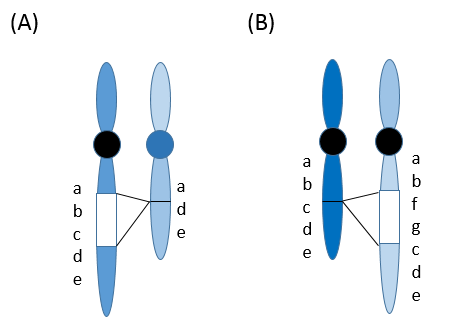
\includegraphics[scale=0.5]{figure2_1}
    \caption[Using NGS to detect deletion, insertion]{
        (A) Deletion is a loss of a segment of DNA;
        (B) Insertion is a type of mutation involving the addition of genetic material.

        }
    \label{fig:Figure2.1}
\end{figure}
    
\item[Single Nucleotide Polymorphism.]

Any two individuals are found to share about 99.9\% identities in
their DNA sequences. Although there is only a small fraction of
genetic variations in the human genome, these variations are often
associated with phenotypic differences and genetic diseases. The
genetic differences between two individuals range from single
point mutations to large structural rearrangements. Single
nucleotide polymorphisms (SNPs) were the most generous category of
genetic variations observed in many species
(Figure~\ref{fig:Figure2.2}(A))~\cite{Frazer2007a,Helmuth2001}. A
set of linked SNPs along the same chromosome is called a haplotype
(Figure~\ref{fig:Figure2.2}(B)). With the development of the
high-throughput SNP genotyping technologies, considerable efforts
have been made to gather haplotype information in human
populations~\cite{Altshuler2005,Chang2006}. For example, the
international HapMap project has provided a haplotype map of about
3.1 million of SNPs across four populations, including 30 trios of
African, 30 trios of European, and 90 Chinese and Japanese
individual~\cite{Frazer2007}. This haplotype map has been widely
used for disease association, population genetics, and
evolutionary analysis, including extent of linkage disequilibrium,
selection of tag
SNPs~\cite{Chang2006,Frazer2007,Huang2008,Huang2005,Huang2005a,Voight2006}.

\begin{figure}
    \centering
    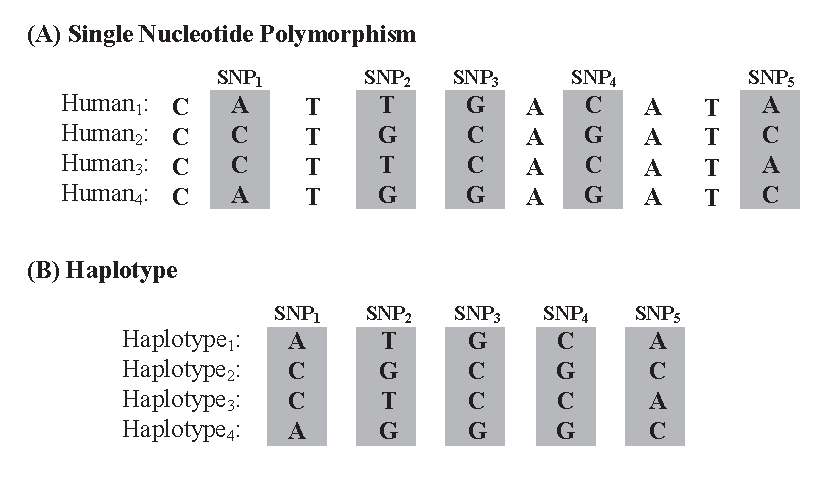
\includegraphics[scale=0.5]{figure2_2}
    \caption[An example for SNPs and haplotypes]{
        (A) A SNP is a single nucleotide in the genome differs between members of a
        species;
        (B) A set of linked SNPs along the same chromosome is called a haplotype.
        }
    \label{fig:Figure2.2}
\end{figure}
    
\end{description}



\section{Introduction to De Novo Assembly}

A critical stage in genome sequencing is the assembly of shotgun reads, o\-r piecing together fragments randomly extracted from the sample, to form a set of contiguous sequences (contigs) representing the DNA in the sample.
Algorithms are available for whole-genome shotgun (WGS) fragment assembly, including: Atlas~\cite{Havlak2004}, ARACHNE~\cite{Batzoglou2002}, Celera, PCAP~\cite{Huang2003}, phrap (http://www.phrap.org), or Phusion~\cite{Mullikin2003}. All these programs rely on the overlap-layout-consensus approach, representing each read as a node and each detected overlap as an edge between the appropriate nodes.
These methods have proved their use through numerous {\em de novo} genome assemblies.

Very short reads are not well suited to this traditional approach. Because of their length, the must be produced in large quantities and at greater coverage depths than traditional Sanger sequencing projects. The sheer number of reads makes the overlap graph, with one node per read, extremely larger and lengthy to compute. With long reads, repeats in the data are disambiguated by careful metrics over long overlaps that distinguish repeat matches from real overlaps, for example, high-quality base disagreements. With short reads, and correspondingly short overlaps to judge from, many reads in repeats will have only a single or no base differences. This leads to many more ambiguous connections in the assembly. However, there are two basic approaches in algorithm for genome assembler: overlap graph and {\em de bruijn} graphs~\cite{Li2012}. These approaches are described below.

\begin{description}

  \item [Overlap Graph.]
  Most established assemblers that were developed for Sanger reads follow the overlap-layout-consensus paradigm. They compute all pair-wise overlaps between the reads and capture this information in graph. Each node in the graph corresponds to a read, and an edge denotes no overlap between two reads (Figure~\ref{fig:Figure2.3}). The overlap graph is used to compute a layout of reads and a consensus sequence of contigs. This method works best when there is a limited number of reads with significant overlap.
  \begin{figure}[ht]
    \centering
    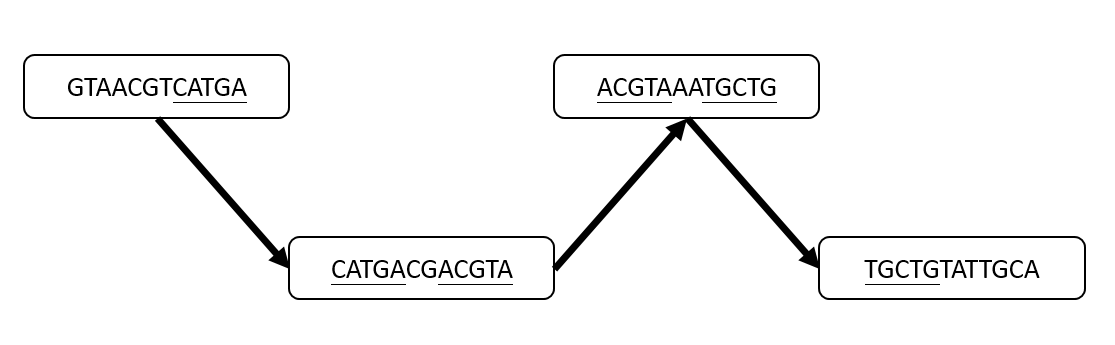
\includegraphics[scale=0.4]{figure2_3}
    \caption[Overlap Graph]{
         Overlap graph of four reads, and underlined nucleotides indicate overlap between reads.
        }
    \label{fig:Figure2.3}
  \end{figure}
  \item [De Bruijn Graph.]
  Because overlap graphs do not scale well with increasing numbers of reads, most assemblers for NGS use {\em de bruijn} graphs. {\em De bruijn} graphs reduce the computational effort by breaking reads into smaller sequences of DNA, called $k$-mers, where the parameter $k$ denotes the length in base of these sequences. The {\em de bruijn} graph captures overlaps of length {\em k-1} between these $k$-mers and not between the actual reads (Figure~\ref{fig:Figure2.4}).
    \begin{figure}[ht]
    \centering
    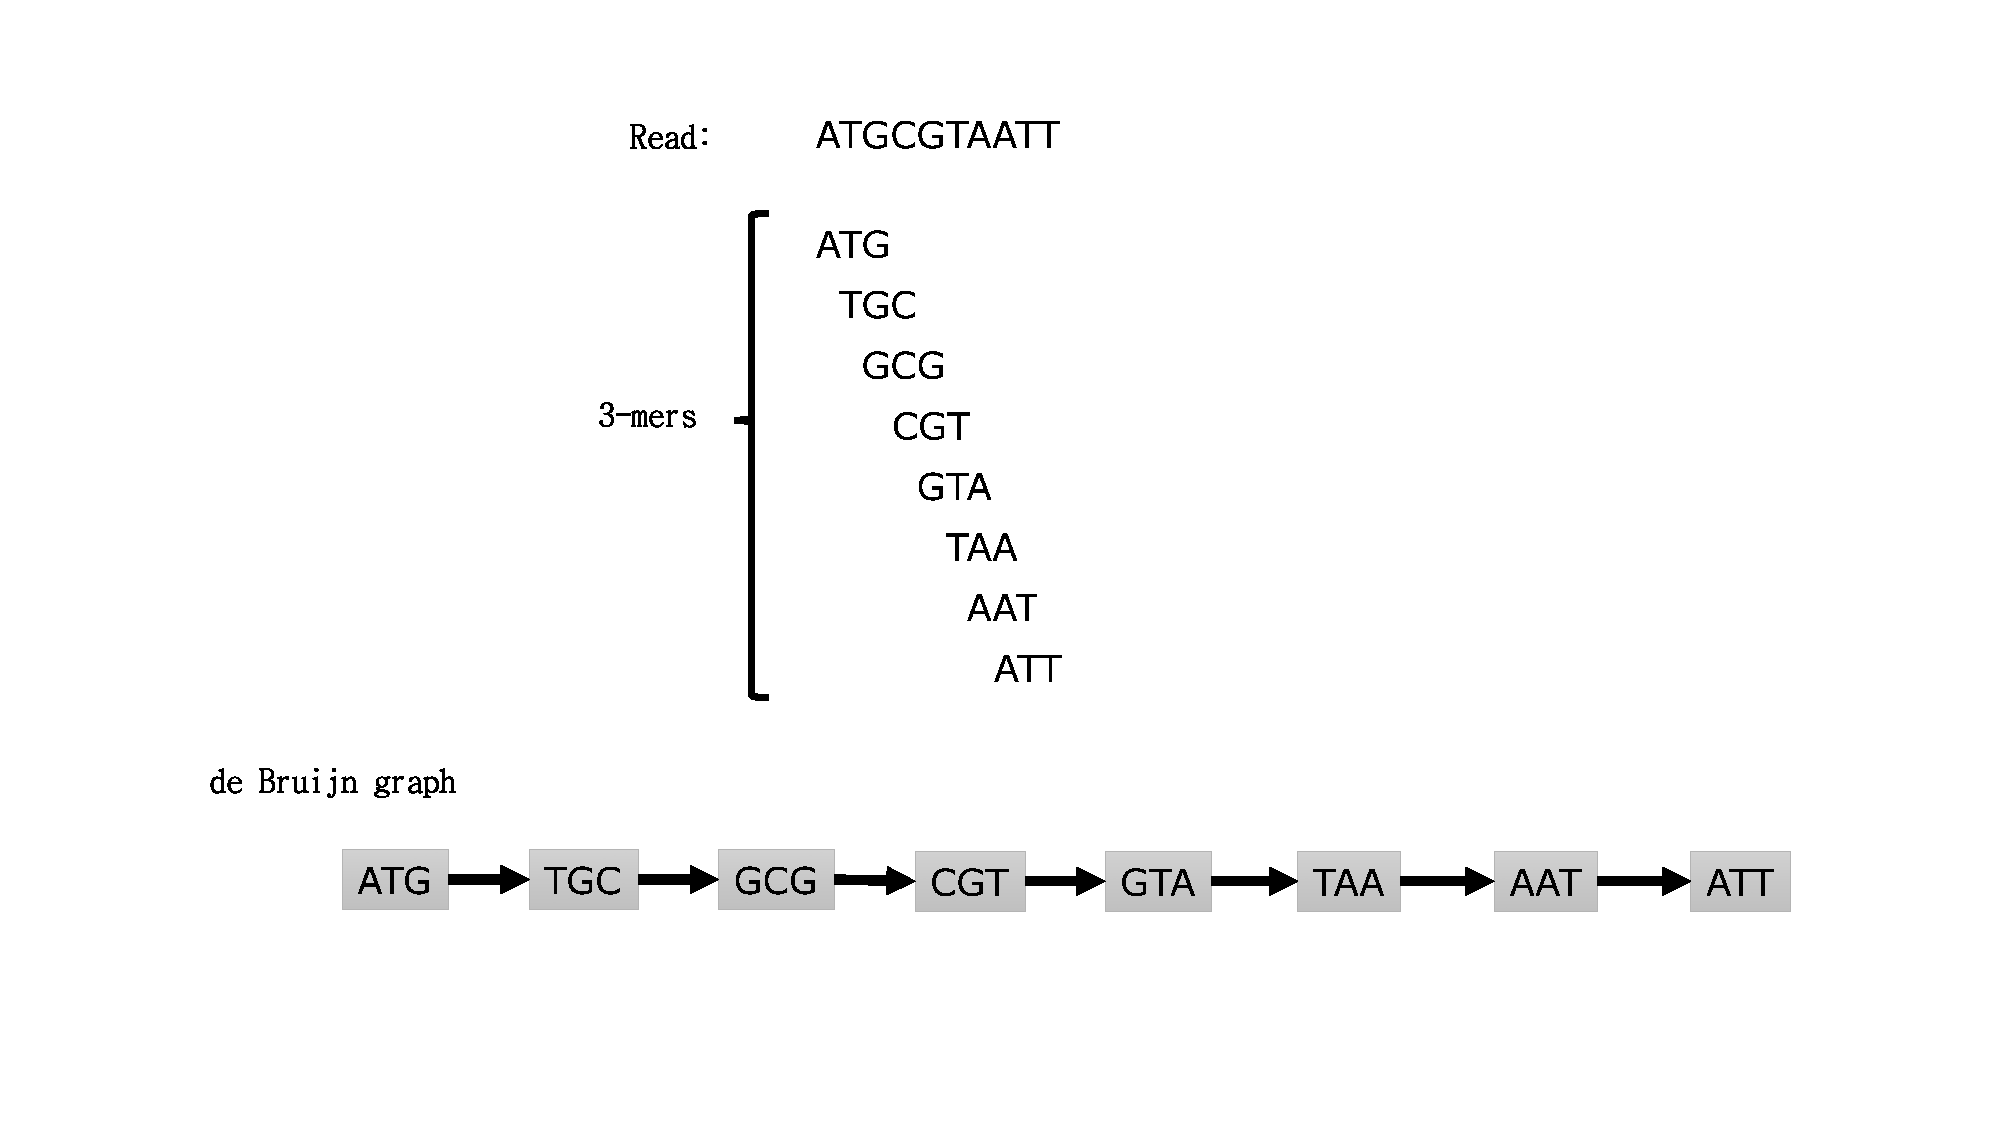
\includegraphics[scale=0.4]{Figure2_4.eps}
    \caption[De Bruijn Graph]{
         De bruijn graph for reads with $k$-mer=3.
        }
    \label{fig:Figure2.4}
  \end{figure}
\end{description}
\paragraph{}
The software package Velvet~\cite{Zerbino2008} was among the first assemblers for short reads and is now widely used. It implements an approach based on {\em de bruijn} graphs, uses information from read pairs, and implements various error correction steps after building the graph. Velvet has successfully been used to assemble bacterial genomes. The assemblers ABySS~\cite{Simpson2009} also use the {\em de bruijn} graph methods. Its advantage is that it can be run in a parallel environment and thus has the potential to assemble much larger genomes. For example, Simpson {\em et al}. demonstrate the assembly of a human genome using ABySS. SOAPdenovo~\cite{Li2008} also implements a parallel assembly algorithm based on {\em de bruijn} graphs. 
 % Background Theory 

\graphicspath{ {Chapters/images/} }
\chapter{Material and Methods}
\section{Overview}

The simulation data sets used Escherichia coli K12 as the reference genome. The donor genome is simulated by randomly placing different sizes of insertions and deletions. Paired-end and mate-pair reads were randomly sheared from the donor genome with coverage 25x via Wgsim from the SAMtools package. The two real data sets are Illumina sequencing data from two rice species (called TN67 and Shio). Both TN67 and Shio have pair-end sequencing with coverage 30x and mate pair sequencing with coverage 100x. The rice reference genome (O. Sativa) is downloaded from the MSU rice genome annotation project.

Our method aims to reconstruct the donor genome by a closely-related reference genome. Potential insertions and deletions (between the reference and donor genomes) are detected using signatures in alignment results of paired-end reads and mate pair reads. Secondly, we assemble detected insertion sequences using a contig graph constructed from paired end reads, and place the insertion or remove deletions from the reference genome to generate a draft genome. Finally, the assembled contigs from paired end reads is used to replace SNPs and indels to reconstruct the donor genome. Figure 3.1 illustrated the flowchart of our method.

\begin{figure}[ht]
\begin{center}
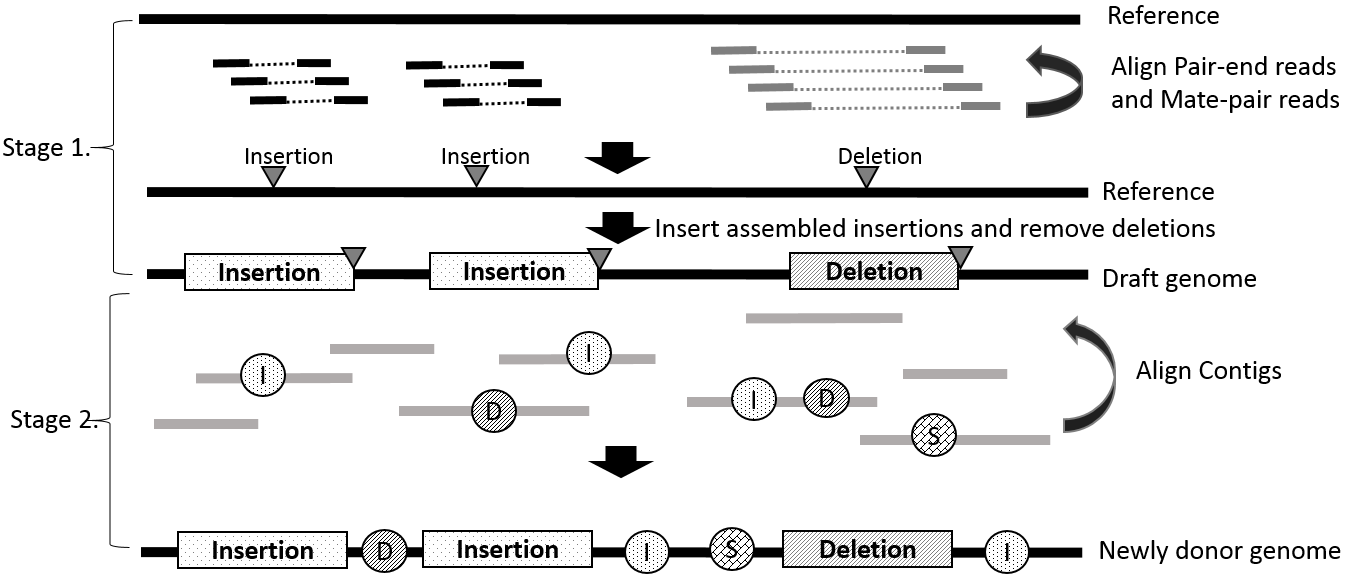
\includegraphics[scale=0.4]{workflow}
\caption{Overview of our method. Stage1: Inserting assembled large-sized insertions and removing deletions to reconstruct a draft genome. Stage2: The draft genome sequence is replaced with the contig sequences, which is able to reflect inter-species SNPs and small-sized indels. Finally, we can get a newly donor genome with large-sized insertions/deletions, small-sized indels, and inter-species SNPs.   }
\label{}
\end{center}
\end{figure}

\newpage
\section{Detection of Potential Insertions and Deletions}

At first, paired-end reads and mate-pair reads of the donor genome separately align onto the closely-related genome via BWA~\cite{BWA}. Several signatures of insertions and deletions can be found in the SAM alignment, including breakpoint reads and aberrant mapping distances (Figure 3.2). 

\begin{figure}[ht]
\begin{center}
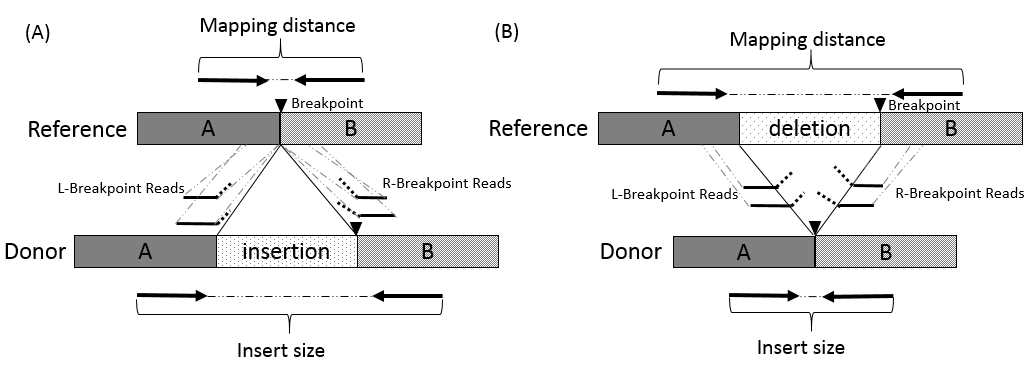
\includegraphics[scale=0.5]{break_signature}
\caption{Paired end reads are aligned to the reference genome. If there exists an insertion or deletion in the donor genome, local alignment of reads nearby the breakpoint are called breakpoint reads. Solid part of breakpoint reads means mapped sequence, and the dashed part of breakpoint reads means unmapped sequence. (A)Insertion. (B)Deletion.}
\label{}
\end{center}
\end{figure}

\subsection{Signatures of Breakpoint Reads}

The breakpoint reads (also called split reads) are reads that span the insertion or deletion loci, and the alignment results of these reads onto a reference often lead to partial local alignments. We further distinguish left and right breakpoint reads according to the position of local alignment with respect to the left or right of the locus. The numbers of left and right breakpoints are defined as $n_l$ and $n_r$.

In practice, owing to repeats, chimera reads, and alignment errors, not all these breakpoint reads are indicative of insertions and deletions. For instance, the numbers of loci containing breakpoint reads can be up to 2,476,410 in the rice genomes. The threshold of minimum $n_l$ and $n_r$ required to call an insertion or deletion is also related to the sequencing coverage. In order to uncover the relation between the threshold and coverage, a number of simulation data sets with different sequencing coverage are conducted. We collected minimum $n_l$ and $n_r$ to estimate the number of breakpoint reads. Linear regression was used to infer the relation between the number of breakpoints $T$ and the sequencing coverage $C$, which is.
\begin{equation} T=1+0.08C
\end{equation}
Since the sequencing coverage $C$ is always known in advance, we can determine the threshold $T$ accordingly. We determine there may be an insertion or a deletion by both the number of left breakpoint reads and the number of right breakpoint reads are larger then $T$. 
\begin{figure}[ht]
\begin{center}
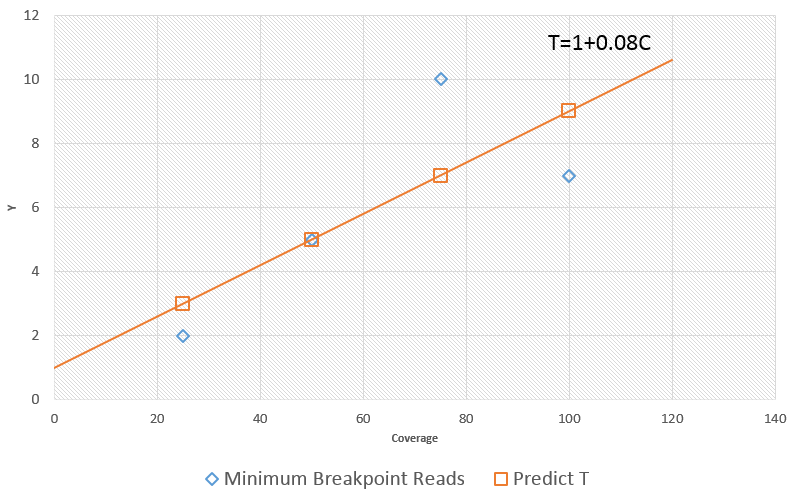
\includegraphics[scale=0.5]{regression}
\caption{A tendency chart about expected T at different coverages.}
\label{}
\end{center}
\end{figure}







\subsection{Signatures of Aberrant Mapping Distance}

Another signature of an insertion or a deletion is aberrant mapping distance between two ends of a read which deviates from the expected distance ($d_e$). By aligning mate pair reads on to the reference genome, an insertion can be detected if mapping distance is smaller than expected insert size. Conversely, if there is a deletion in the donor genome, the mapping distance is larger than expected insert size. For each breakpoint, we collect the mapping distances of mate pair reads with two ends across each breakpoint $b_i$. The median of mapping distances across each breakpoint is defined as ($d_{b_i}$) (see Figure 3.3). 


\begin{figure}[ht]
\begin{center}
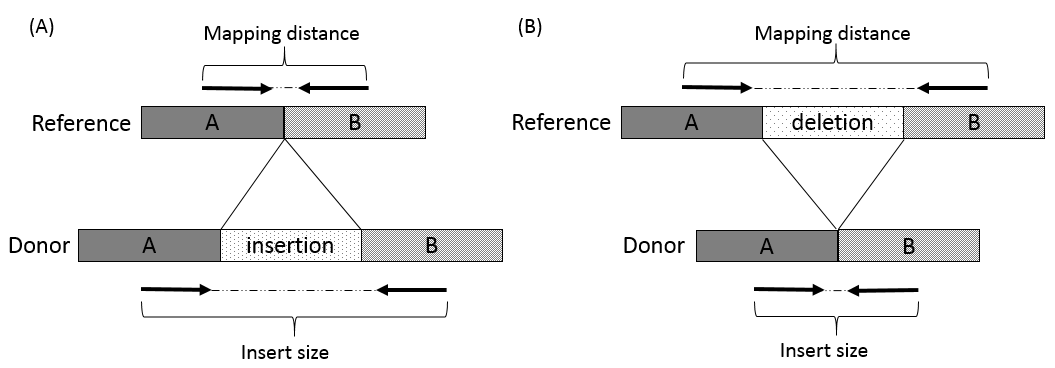
\includegraphics[scale=0.5]{mapping}
\caption{Mate pair reads are aligned to the reference genome.(A)If there is an insertion in the donor genome, mapping distance is smaller than the insert size; (B)If there is a deletion in the donor genome, mapping distance is larger than the insert size.   }
\label{}
\end{center}
\end{figure}


\subsection{Identification of Insertions and Deletions}

    In practice, we first identify all the genomic loci with $n_r > T$. Note that we can't know if each locus is insertion or deletion at this moment. Subsequently, the median of mapping distance $d_{b_i}$ is computed and compared against $d_e$. This position is considered as insertion if $d_{b_i}<d_e$. Otherwise ($d_{b_i}>d_e$), it is considered as deletion.  

    Furthermore, the number of reads fully aligned across the breakpoint ($nf_{b_i}$) should be as few as possible. And the left breakpoint reads $n_l$ should be greater than $T$. In summary, an insertion or deletion is called if satisfying all the following rules: (1) $nl_{b_i} > T$ and $nr_{b_i} > T$, (2) $nf_{b_i}$, and (3) $d_{b_i} < d_e$. 

    The length of insertions is estimated by $D_e$ minus $D_m$. Although deletions can be estimated in similar way, it can be precisely computed by the distance between the left and right breakpoint loci, which are exactly the same as the deletion size (see Figure 3.4). 


\begin{figure}[ht]
\begin{center}
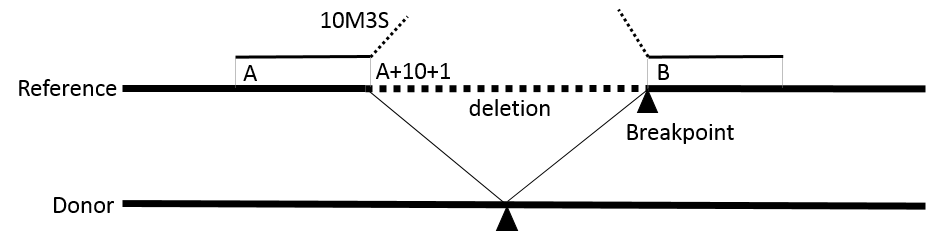
\includegraphics[scale=0.5]{Deletion_range}
\caption{ A left breakpoint read which CIGAR is 10M3S at position A, and the breakpoint at position B. The range of the deletion is A+10+1 to B-1. }
\label{}
\end{center}
\end{figure}

\newpage
\section{Assembly of Insertion Sequences}

Although the insertion loci can be inferred using the above method, the insertion sequences are not reconstructed. In order to assemble these insertion sequences, we solve a local assembly problem using a contig graph generated by SGA. The first step aims to map the left/right sequences flanking each insertion onto vertices in the graph. The second step aims to reconstruct the insertion sequence from contig graph.

\subsection{Mapping of Insertion Flanking Sequences onto Contig Graph}

Paired-end reads are assembled to contigs by SGA, which outputs a contig sequences and a contig graph (Figure 3.5). Subsequently, we extract one left and one right sequences flanking each insertion locus (called L-Read and R-Read), and map the two sequences onto the contig graph via the following procedure. 

The mapping procedure relies on an FM-index constructed from contig sequences (assembled by SGA~\cite{Simpson2012a}). Each pair of L-Read and R-Read are mapped onto the contig sequences (containing them as substrings) using the backward-search algorithm~\cite{Ferragina2000}. 

If both L-Read and R-Read are mapped onto same vertex in the contig graph, the sequence of the insertion is return. Otherwise, we try to find paths between the two vertices that L-Read mapped (called start vertex) and the contig that L-Read mapped (called end vertex) on the contig graph. By performing breadth-first search of contigs, we reconstruct the sequence of insertions.



\begin{figure}[ht]
\begin{center}
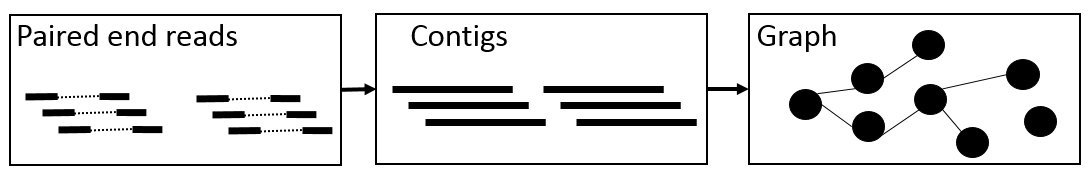
\includegraphics[scale=0.5]{contig_graph}
\caption{Paired-end reads are assembled to contigs. And then, using these assembled contigs to construct a contig graph.}
\label{}
\end{center}
\end{figure}

\begin{figure}[ht]
\begin{center}
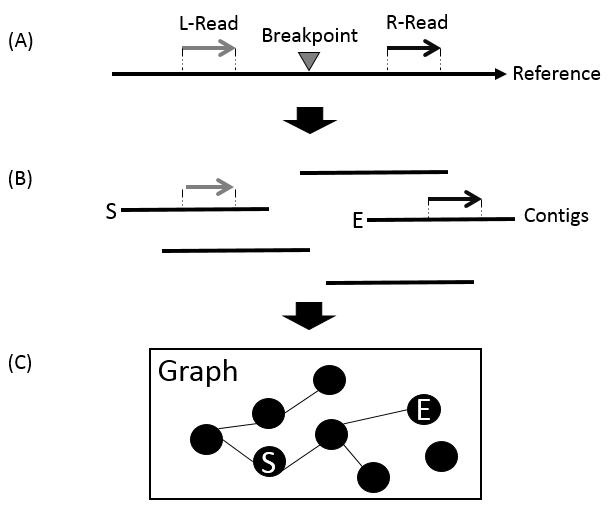
\includegraphics[scale=0.5]{align_readtocontig}
\caption{}
\label{}
\end{center}
\end{figure}

\newpage

\subsection{Breadth First Search of Insertion Sequence}

Given a start vertex and an end vertex on the contig graph, we use the algorithm findwalks of SGA to search paths between start contig and end contig. Assembly is performed by traversing the contig graph in a breadth-first search order from a given start vertex. The process stop while the maximum distance (set to sum of predict length, start vertex size and end vertex size) between the start vertex and the end vertex is reached, or the maximum number of leaves (set to 3000k) is reached. 

When traversing the contig graph, it records the paths while the expended node is the end vertex. Get the sequences from all recorded paths present, we select one of these sequence which length is closest to the predict length of the insertion. And then,we can return the sequence as insertion sequence. It means that the absolute value of the predict length minus path length is minimum. 

By using predict length of insertion, we will find the more correct path from all possible paths. For example, if the insertion contains two repeats, it may construct a path containing one repeat and a path containing two repeats. As the result, the predict length is helpful for selecting the path containing two repeats(See Figure 3.7). If no path that can reach end vertex from start vertex, the insertion is assembled unsuccessfully. 




\begin{figure}[ht]
\begin{center}
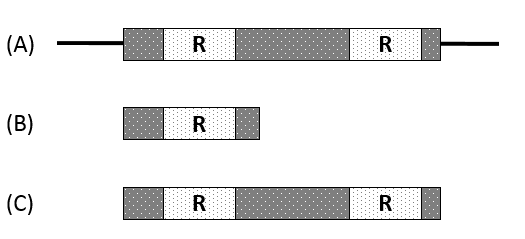
\includegraphics[scale=0.5]{repeat_insertion}
\caption{(A) is the real insertion contains repeats R. (B) and (C) are two assembled insertions from two possible paths. Using predict length of insertion, we can select (C) not (B).  }
\label{}
\end{center}
\end{figure}

\section{Alignment of Contigs to the Draft Genome}

We can generate a draft genome after placing large-sized insertions and removing deletions from the reference genome. Although we can detect and assemble large-sized insertions and range of deletions, there are SNPs and small indels between the donor genome and the closely-related reference genome. SNPs and indels are easy to construct by assembling reads to contigs because they could be generated into assembled contigs. So, we align assembled contigs onto the draft genome. SNPs and indels will be filled into the draft genome with the aligned portions of these contigs by parsing the SAM alignment results.

At first, the SAM alignment results are sorted by the alignment positions. And then, we substitute the aligned portion of the contig for draft genome while the end position of the aligned portion of the contig is larger than previous contig, conversely, we skip this alignment result. Figure3.8 illustrate the way to substitute the aligned portion by aligned contigs.
Finally, the draft genome sequence is replaced with the contig sequences, which is able to reflect inter-species SNPs and small-sized indels.

\begin{figure}[ht]
\begin{center}
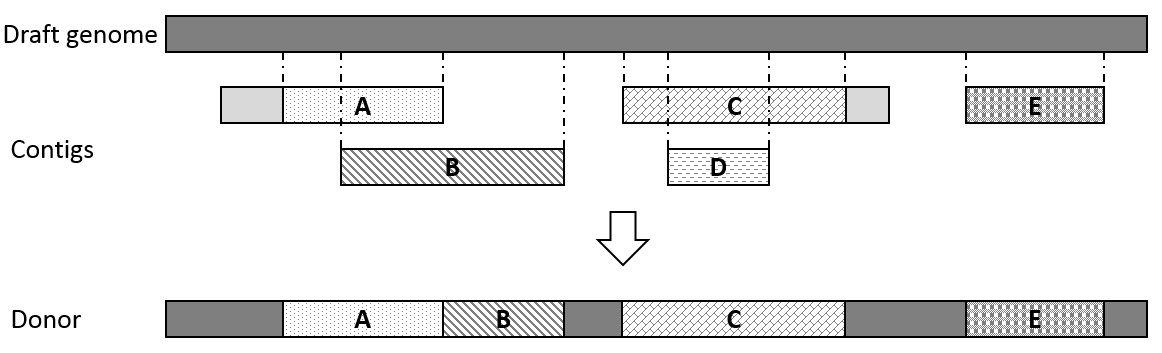
\includegraphics[scale=0.4]{contig_align}
\caption{The SAM alignment results of contigs are sorted with the alignment position. The dash lines show the aligned portion of each contig. At first, we substitute the aligned portion of contig A for the aligned portion of reference genome. Secondly, we substitute partly aligned portion of contig B for the aligned portion of the reference genome because the start aligned position of contig B is smaller than the end aligned position of contig A. And then, we process contig C and E. The result of skipping contig D is that the end aligned position of contig D is smaller than the end aligned position of contig C. Finally, we get a newly donor genome after all the contigs are done.}
\label{}
\end{center}
\end{figure}

















 % Experimental Setup

\graphicspath{ {Chapters/images/} }
\chapter{Result And Discussion}

We test accuracy and detection power of our method called SemiAssembler in comparison with MindTheGap using a variety of simulations and real sequencing data. MindTheGap is specific for the detection and assembly of insertions, and thus only insertions can be compared with MindTheGap.   
The simulation data sets used Escherichia coli K12 as the reference genome, whereas paired-end reads (insert size 450bp) and mate pair reads (insert size 4.5kb) are randomly sheared by wgsim. Real sequencing data sets are from two rice species (called TN67 and Shio),and $O. Sativa$ is used as the reference genome. Paired-end (with insert size 400bp) and mate-pair (with insert size 3kb) libraries were constructed and sequenced. These paired-end and mate-pair reads were separately aligned onto the reference genome using BWA-aln to produce standard SAM alignments, which are the input of our method. Paired-end reads and reference genome sequence are the input of MindTheGap. Table 4.1 shows the information of simulated data and real sequencing data. 

\begin{table}[!ht]
    \centering
    \begin{tabular}[t]{l|c|c|c|}
      & Simulated data set & Real data set & Real data set  \\
      \hline
      Species & {E.coli} & {TN67} & {Shio} \\
      Reference & E.coli &  \multicolumn{2}{|c|}{O. Sativa} \\     
      \cline{3-4}
      Genome Size & 4,641,653 bp &  \multicolumn{2}{|c|}{373,245,519 bp} \\
      \cline{3-4}
      Coverage of Paired-end & 25x & 33x & 33x \\
      Insert size of Paired-end & 450 & 450 & 450 \\
      Coverage of Mate-pair & 25x & 106x & 108x \\
      Insert size of Mate-pair & 4500 & 3672 & 4001 \\
      Number of Insertions & 30 & 6 & 3 \\ 
      Number of Deletions & 30 & 5 & 9 \\ 

      
   \end{tabular}
    \caption{}
    \label{}
\end{table}


\section{Results On Simulated Data Sets}


In order to understand the accuracy and power of our method  with respect to different sizes of insertions and deletions, we carried out several simulations at 25x coverage for each experiment. Only insertions will be compared with MindTheGap, which does not identify deletions.  

We simulate 30 insertions for each experiment. Figure 4.1 and Figure 4.2 illustrate the results of simulations with different sizes of insertions at 25x coverage. The detection power of SemiAssembler is less than that of MindTheGap, while both methods achieve the same precision. In terms of the assembled insertion sequences (Figure 4.4), the insertions assembled by our method is more accurate than that of MindTheGap. 
In terms of deletions, we also simulate 30 deletions for each experiment. Figure 4.5 illustrate the results of simulations with different sizes of deletions at 25x coverage. Even though we can not detect all insertions, SemiAssembler is still able to find most of the insertions ($>80$\%) with high accuracy.



\begin{figure}[ht]
\begin{center}
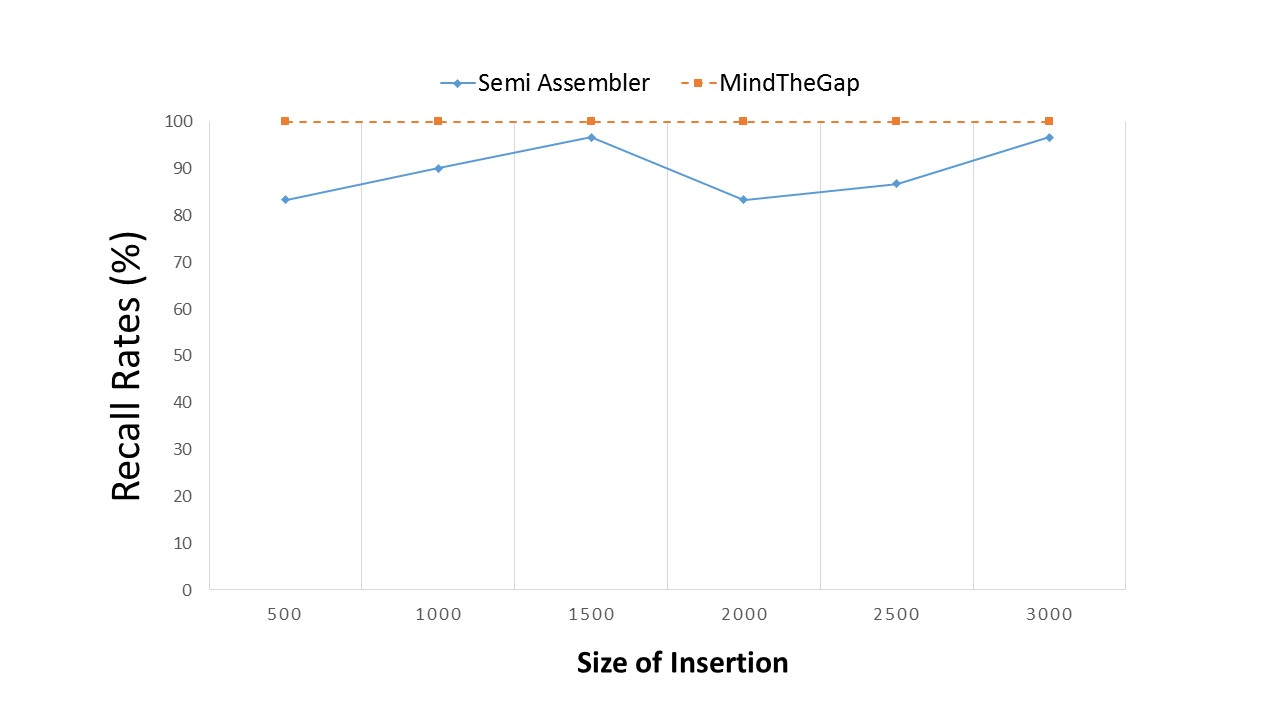
\includegraphics[scale=0.4]{r_recall2}
\caption{Recall rates of detecting insertions with different sizes. SemiAssembler can detect the insertions with high recall rates ($>80$\%).}
\label{}
\end{center}
\end{figure}

\begin{figure}[ht]
\begin{center}
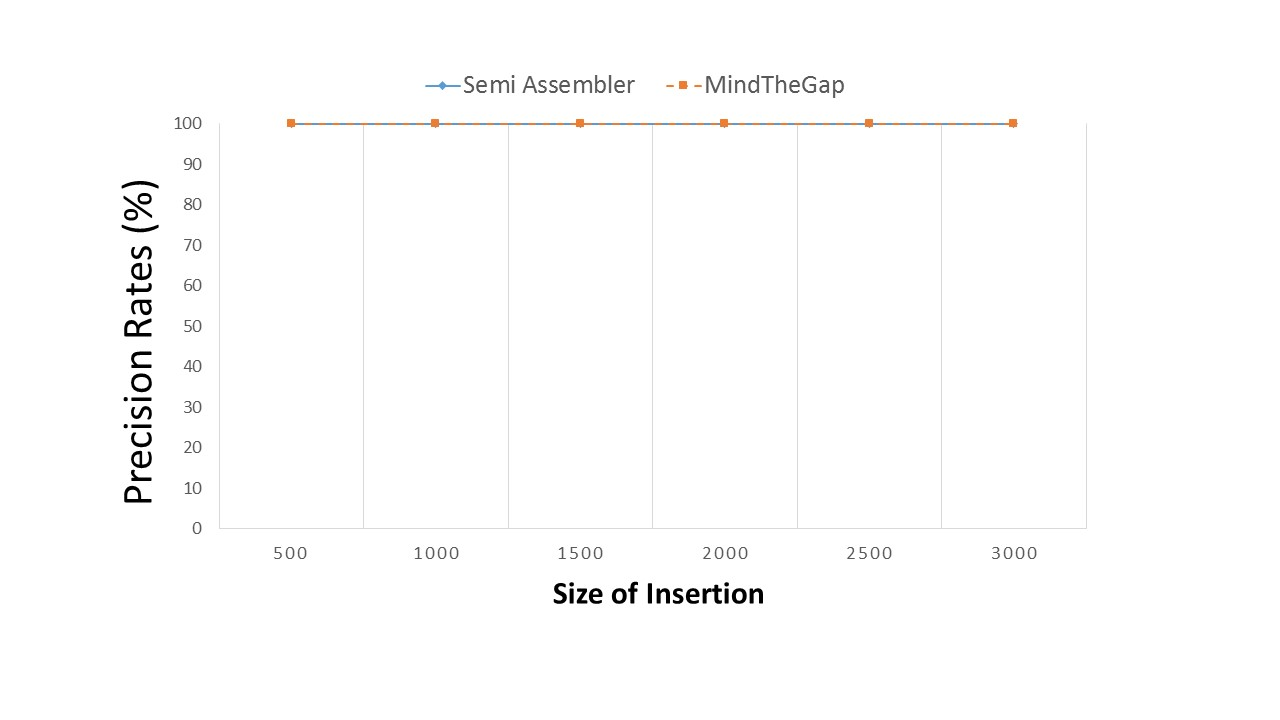
\includegraphics[scale=0.4]{r_prec}
\caption{Precision rates of detecting insertions with different sizes.}
\label{}
\end{center}
\end{figure}

\begin{figure}[ht]
\begin{center}
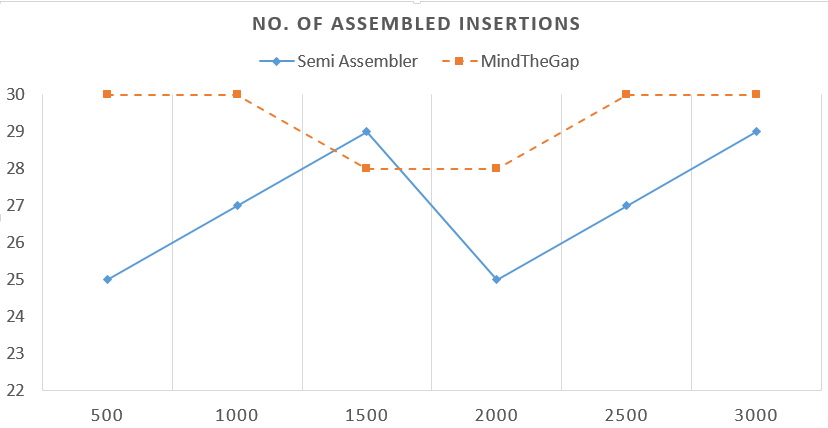
\includegraphics[scale=0.5]{r_assemble}
\caption{Number of assembled insertions.}
\label{}
\end{center}
\end{figure}

\begin{figure}[ht]
\begin{center}
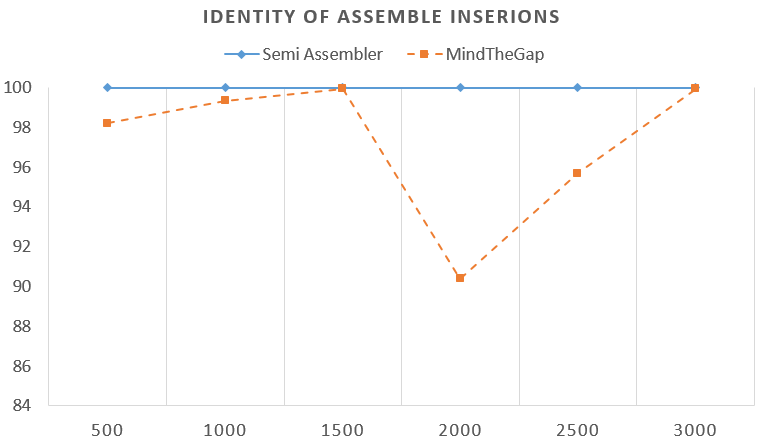
\includegraphics[scale=0.5]{r_id}
\caption{Identity of assembled insertions. SemiAssembler can assemble insertions with higher identities.}
\label{}
\end{center}
\end{figure}

\begin{figure}[ht]
\begin{center}
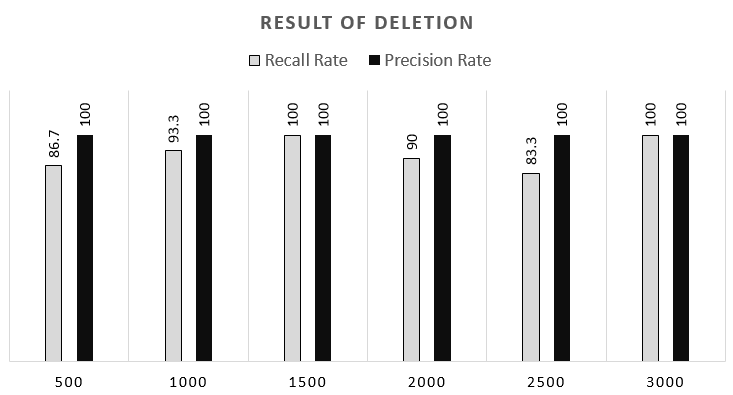
\includegraphics[scale=0.5]{deletion_result}
\caption{Simulated deletions of different sizes. SemiAssembler can detect the deletions ($>80$\%) with high accuracy.}
\label{}
\end{center}
\end{figure}




\clearpage


\section{Results On Real Sequencing Data Set}
We use real sequencing data sets of two rice species (called TN67 and Shio) to evaluate SemiAssembler. Sequencing data of TN67 and Shio are two related species derived from $O. Sativa$, in which the reference genome can be downloaded from the MSU rice genome annotation project. 

\subsection{Results of Detection of Large-sized Insertions}
We totally detect 403 insertions in TN67, and 273 insertions can be assembled. In Shio, we totally detect 190 insertions and assemble 127 insertions. We also run MindTheGap using the same data sets and compare the results with our method. MindTheGap totally detect 27344 insertions in TN67, and 5046 insertions can be assembled. In Shio, MindTheGap totally detect 23148 insertions, and 3582 insertions can be assembled. The total number of detected insertions with running MindTheGap is larger than our method because MindTheGap can detect small indels and our method detect large-sized insertions in this stage. Although we can not detect small insertions in this stage, we reflect small insertions/deletions and SNPs in the final stage of our method by using assembled contigs. 

In order to understand the accuracy and power of SemiAssembler, we use several validated large-sized insertions. Six insertions in TN67 and three insertions in Shio are detected by our method and validated by PCR and Sanger sequenced. Table 4.2 lists the number of detected and assembled insertions of both methods for TN67 and Shio.  In our mehod, we can detect all the nine insertions and assemble seven of them. On the other hand, MindTheGap can only detect seven insertions and assemble four of them. Most of these insertion sequences are composed of complex repeats difficult to be assembled. 



\subsection{Results of Detection of Large-sized Deletions}
In terms of deletions, we totally detect 422 deletions in TN67 and 353 deletions in Shio. We also use validated deletions to understand the accuracy and power of SemiAssembler. Three large-size deletions in TN67 and eight large-size deletions in Shio were validated by PCR and Sanger sequencing. We can detect 2 deletions in TN67 and 7 deletions in Shio. The two undetected deletions are due to the number of breakpoint reads is less than the default threshold (default 3). Table 4.2 list the results of detection of deletions for TN67 and Shio.


\begin{table}[!ht]
    \centering
    \begin{tabular}[t]{l|llll|ll}
   Species  & Method & No. of  & TP & Assembled  &  No. of & TP\\
             &        &Insertions    & &Insertions  & Deletions & \\
      \hline
      
     TN67 & SemiAssembler & 6 & 6 & 5 & 3 & 2\\
     TN67  & MindTheGap & 6 & 4 & 2 & - & -\\
     Shio & SemiAssembler & 3 & 3 & 2 & 8 & 7\\
     Shio  & MindTheGap & 3 & 3 & 2 & - & -\\

      
   \end{tabular}
    \caption{The number of validated insertions is in the column 'No. of Insertions'. The number of validated deletions is in the column 'No. of Deletions'.}
    \label{}
\end{table}



\subsection{Results of Detection of Indels}

Because the number of small indels is relatively large, the Sanger sequencing were not conducted and the exact sizes of these indels are not known. Nevertheless, as gel electrophoresis can separate DNA fragments based on their sizes, we can still compare the relative indel sizes between TN67 and Shio with those predicted by our method. For instance (see Figure 4.6), the indel at this locus of TN67 is larger than that of Shio.

\begin{figure}[ht]
\begin{center}
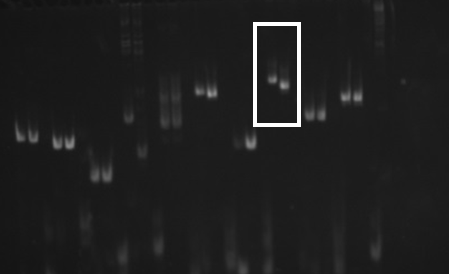
\includegraphics[scale=0.5]{ssr_screen}
\caption{Larger molecules move more slowly through the gel while the smaller molecules move faster. TN67 is on the left,and Shio is on the right in this gel electrophoresis.}
\label{}
\end{center}
\end{figure}

The major advantage of SemiAssembler is the assembled genome which is able to reflect small SNPs and indels across different species. Therefore, a subset of commonly-used biomarkers (from http://archive.gramen\-e.org/markers/microsat/) were screened using PCR in the TN67 and Shio genomes. 
These 75 biomarkers represent small indels ranging approximately from 1bp to 18bp. The gel electrophoresis shows that 42 of them may have indels between TN67 and Shio. In our method, we can recover 12 small insertions and 10 small deletions from these 42 small indel regions. On the other hand, MindTheGap can only detect one insertion from these 42 indels, and the only one detected insertion failed to be assembled. Table 4.4 list the results of detection of indels for TN67 and Shio.

\hfill
\begin{table}[!ht]
    \centering
    \begin{tabular}[t]{l|llll}
     Species & Method &  No. of Indels & Insertion & Deletion\\\\
      \hline
      
    TN67 & SemiAssembler & 12 & 8 & 4 \\
    TN67 & MindTheGap & 1 & 1 & - \\
    Shio & SemiAssembler & 10 & 1 & 9 \\
    Shio & MindTheGap & 0 & 0 & - \\\\
      
   \end{tabular}
    \caption{The result of recovering small indels in 42 validated small indels. The number of detected indels is in the column 'N'.}
    \label{}
\end{table}



 % Experiment 1

\graphicspath{ {Chapters/images/} }
\chapter{Conclusion and Future Work}
\section{Conclusion}
In recent years, several reference-mapping approaches detect only small-sized or large-sized structural variants(SVs) and only report locus of SVs. {\em De novo} assembly has the advantage of assembling SVs but the genomes assembled are often fragmented into large numbers of contigs.

In this paper, we design a semi-assembly approach called SemiAssembler which integrate reference-mapping approaches and {\em de novo} assembly to reconstruct a newly-sequenced genome using closely-related reference genome. We can generate a draft genome with large-sized insertions and deletions, and then we replace draft genome sequence with contigs to reflect inter-species SNPs and small-sized indels. The results of assembled newly-sequenced genome indicate that the genome assembled not only provides better contiguity but also uncover a substantial amount of inter-species variations.

\section{Future Work}
We can not find all insertions and deletions in our method because the number of breakpoint reads is less than the default threshold. The default threshold is set by average coverage, so the variance between coverages is a big issue.
 % Experiment 2



%\input{Chapters/Chapter7} % Conclusion

%% ----------------------------------------------------------------
% Now begin the Appendices, including them as separate files

\addtocontents{toc}{\vspace{2em}} % Add a gap in the Contents, for aesthetics
\appendix % Cue to tell LaTeX that the following 'chapters' are Appendices
\graphicspath{ {Chapters/images/} }
\chapter{Supplementary Tables}


\begin{table}[!ht]
    \centering
    \begin{tabular}[t]{l|llll}
      & Species (loci) & Insertion Size & Detection & Assembly \\\\
      \hline
      
     SemiAssembler & TN67(Chr3:29074003)  & 1404 & YES & NO \\
     MindTheGap & TN67(Chr3:29074003)  & 1404 & YES & NO \\\\
     SemiAssembler & TN67(Chr5:15076333)  & 1273 & YES & YES \\
     MindTheGap & TN67(Chr5:15076333)  & 1273 & YES & NO \\\\
     SemiAssembler & TN67(Chr6:2528106)  & 1396 & YES & YES \\
     MindTheGap & TN67(Chr6:2528106)  & 1396 & YES & YES \\\\
     SemiAssembler & TN67(Chr6:9338026)  & 1901 & YES & YES \\
     MindTheGap & TN67(Chr6:9338026)  & 1404 & NO & NO \\\\
     SemiAssembler & TN67(Chr6:10870313)  & 1353 & YES & YES \\
     MindTheGap & TN67(Chr6:10870313)  & 1353 & NO & NO \\\\
     SemiAssembler & TN67(Chr11:19708716)  & 563 & YES & YES \\
     MindTheGap & TN67(Chr11:19708716)  & 563 & YES & YES \\\\
     SemiAssembler & Shio(Chr1:28591586)  & 1848 & YES & YES \\
     MindTheGap & Shio(Chr1:28591586)  & 1848 & YES & YES \\\\
     SemiAssembler & Shio(Chr3:29074003)  & 1401 & YES & NO \\
     MindTheGap & Shio(Chr3:29074003)  & 1401 & YES & NO \\\\
     SemiAssembler & Shio(Chr11:19708716)  & 563 & YES & YES \\
     MindTheGap & Shio(Chr11:19708716)  & 563 & YES & YES \\\\
     
     


      
   \end{tabular}
    \caption{The results of detecting large-sized insertions in real data sets.}
    \label{}
\end{table}


\hfill
\begin{table}[!ht]
    \centering
    \begin{tabular}[t]{l|llll}
     Species & Deletion Range & Size & Detection\\\\
      \hline
      
     TN67  & Chr4:18316281-18317704 & 1423 & YES\\\\
     TN67  & Chr7:201825-202859 & 1034 & NO\\\\
     TN67  & Chr8:15081572-15082776 & 1204 & YES\\\\
     Shio  & Chr1:1682294-1684032 & 1738 & YES\\\\
     Shio  & Chr4:4034161-4037128 & 2967 & YES\\\\
     Shio  & Chr4:4390578-4392017 & 1439 & YES\\\\
     Shio  & Chr7:24442070-24442350 & 280 & YES\\\\
     Shio  & Chr8:5391784-5393686 & 1902 & NO\\\\
     Shio  & Chr8:15081572-15082776 & 1204 & YES\\\\
     Shio  & Chr10:11842024-11842248 & 224  & YES\\\\
     Shio  & Chr11:22937697-22937979 & 282 & YES\\\\


      
   \end{tabular}
    \caption{The results of detecting large-sized deletions in real data sets.}
    \label{}
\end{table}






%\input{Appendices/AppendixA}	% Appendix Title

%\input{Appendices/AppendixB}    % Appendix Title

%\input{Appendices/AppendixC} % Appendix Title

\addtocontents{toc}{\vspace{2em}}  % Add a gap in the Contents, for aesthetics
\backmatter


%% ----------------------------------------------------------------
\label{Bibliography}
\lhead{\emph{Bibliography}}  % Change the left side page header to "Bibliography"
\bibliographystyle{unsrtnat}  % Use the "unsrtnat" BibTeX style for formatting the Bibliography
\bibliography{Bibliography}  % The references (bibliography) information are stored in the file named "Bibliography.bib"

\end{document}  % The End
%% -------------------------------------------------------------
\appendix % Cue to tell LaTeX that the following 'chapters' are Appendices
\graphicspath{ {Chapters/images/} }
\chapter{Supplementary Tables}


\begin{table}[!ht]
    \centering
    \begin{tabular}[t]{l|llll}
      & Species (loci) & Insertion Size & Detection & Assembly \\\\
      \hline
      
     SemiAssembler & TN67(Chr3:29074003)  & 1404 & YES & NO \\
     MindTheGap & TN67(Chr3:29074003)  & 1404 & YES & NO \\\\
     SemiAssembler & TN67(Chr5:15076333)  & 1273 & YES & YES \\
     MindTheGap & TN67(Chr5:15076333)  & 1273 & YES & NO \\\\
     SemiAssembler & TN67(Chr6:2528106)  & 1396 & YES & YES \\
     MindTheGap & TN67(Chr6:2528106)  & 1396 & YES & YES \\\\
     SemiAssembler & TN67(Chr6:9338026)  & 1901 & YES & YES \\
     MindTheGap & TN67(Chr6:9338026)  & 1404 & NO & NO \\\\
     SemiAssembler & TN67(Chr6:10870313)  & 1353 & YES & YES \\
     MindTheGap & TN67(Chr6:10870313)  & 1353 & NO & NO \\\\
     SemiAssembler & TN67(Chr11:19708716)  & 563 & YES & YES \\
     MindTheGap & TN67(Chr11:19708716)  & 563 & YES & YES \\\\
     SemiAssembler & Shio(Chr1:28591586)  & 1848 & YES & YES \\
     MindTheGap & Shio(Chr1:28591586)  & 1848 & YES & YES \\\\
     SemiAssembler & Shio(Chr3:29074003)  & 1401 & YES & NO \\
     MindTheGap & Shio(Chr3:29074003)  & 1401 & YES & NO \\\\
     SemiAssembler & Shio(Chr11:19708716)  & 563 & YES & YES \\
     MindTheGap & Shio(Chr11:19708716)  & 563 & YES & YES \\\\
     
     


      
   \end{tabular}
    \caption{The results of detecting large-sized insertions in real data sets.}
    \label{}
\end{table}


\hfill
\begin{table}[!ht]
    \centering
    \begin{tabular}[t]{l|llll}
     Species & Deletion Range & Size & Detection\\\\
      \hline
      
     TN67  & Chr4:18316281-18317704 & 1423 & YES\\\\
     TN67  & Chr7:201825-202859 & 1034 & NO\\\\
     TN67  & Chr8:15081572-15082776 & 1204 & YES\\\\
     Shio  & Chr1:1682294-1684032 & 1738 & YES\\\\
     Shio  & Chr4:4034161-4037128 & 2967 & YES\\\\
     Shio  & Chr4:4390578-4392017 & 1439 & YES\\\\
     Shio  & Chr7:24442070-24442350 & 280 & YES\\\\
     Shio  & Chr8:5391784-5393686 & 1902 & NO\\\\
     Shio  & Chr8:15081572-15082776 & 1204 & YES\\\\
     Shio  & Chr10:11842024-11842248 & 224  & YES\\\\
     Shio  & Chr11:22937697-22937979 & 282 & YES\\\\


      
   \end{tabular}
    \caption{The results of detecting large-sized deletions in real data sets.}
    \label{}
\end{table}




 % Results and Discussion